\documentclass{article}
\usepackage[final]{nips_2017}

% to compile a camera-ready version, add the [final] option, e.g.:
% \usepackage[final]{nips_2017}

\usepackage[utf8]{inputenc} % allow utf-8 input
\usepackage[T1]{fontenc}    % use 8-bit T1 fonts
\usepackage{hyperref}       % hyperlinks
\usepackage{url}            % simple URL typesetting
\usepackage{booktabs}       % professional-quality tables
\usepackage{amsfonts}       % blackboard math symbols
\usepackage{nicefrac}       % compact symbols for 1/2, etc.
\usepackage{microtype}      % microtypograph

\usepackage{graphicx}
\usepackage{amsmath}

\bibliographystyle{plain}

\title{Reproduction: Unsupervised Monocular Depth Estimation with Left-Right Consistency}

% The \author macro works with any number of authors. There are two
% commands used to separate the names and addresses of multiple
% authors: \And and \AND.
%
% Using \And between authors leaves it to LaTeX to determine where to
% break the lines. Using \AND forces a line break at that point. So,
% if LaTeX puts 3 of 4 authors names on the first line, and the last
% on the second line, try using \AND instead of \And before the third
% author name.

\author{
	Andrija Djurisic\\
	Faculty of Mathematics, Belgrade\\
	\texttt{andrija.m.djurisic@gmail.com} \\
	%% examples of more authors
	%% \And
	%% Coauthor \\
	%% Affiliation \\
	%% Address \\
	%% \texttt{email} \\
	%% \AND
	%% Coauthor \\
	%% Affiliation \\
	%% Address \\
	%% \texttt{email} \\
	%% \And
	%% Coauthor \\
	%% Affiliation \\
	%% Address \\
	%% \texttt{email} \\
	%% \And
	%% Coauthor \\
	%% Affiliation \\
	%% Address \\
	%% \texttt{email} \\
}

% * describe each loss
% * your own observations about the paper, e.g. analysis of robustness, was the paper difficult to reproduce given the details in the paper; most important tricks in
% implementation etc. 
% * One thing I can do to improve training time overall is to introduce data loading pipeline by using tf.data.
% * I havent trained on CS
% * I havent do any data augmentation

\begin{document}
	% \nipsfinalcopy is no longer used
	
	\maketitle
	
%	\begin{abstract}
%		The abstract paragraph should be indented \nicefrac{1}{2}~inch
%		(3~picas) on both the left- and right-hand margins. Use 10~point
%		type, with a vertical spacing (leading) of 11~points.  The word
%		\textbf{Abstract} must be centered, bold, and in point size 12. Two
%		line spaces precede the abstract. The abstract must be limited to
%		one paragraph.
%	\end{abstract}
	
\section{Introduction}
In this paper Godard et. al. \cite{DBLP:journals/corr/GodardAB16} are presenting unsupervised method for solving depth estimation problem. 

%Most existing approaches treat depth estimation as a supervised regression problem and as a result, require vast quantities of corresponding ground truth depth data for training.

The most learning based methods for monocular depth estimation rely on the availability of ground truth depth data aligned with each input image. These methods take color-depth pairs as an input during the training and learn to directly predict depth maps from color images. One such method is \emph{DispNet} \cite{DBLP:journals/corr/MayerIHFCDB15} which introduced fully convolutional architecture similar to one used in this paper. 

Capturing reliable depth data is both expensive and time-consuming and as an alternative stereo data is much easier to capture requiring only two synchronized cameras. Authors are proposing novel method which takes color image captured from the left camera as an input and color image captured from the right camera as a target during the training. Their convolutional neural network then learns to generate per pixel disparities that produce the right target image by shifting pixels from the left input image using differentiable image sampler. Depth can be then trivially recovered from the predicted disparity.

% Depth tells us how much each pixel moves between the images in a stereo pair.

\section{Method}
At training time, we have access to two images $I^l$ and $I^r$, corresponding to the left and right color images from a calibrated stereo pair, captured at the same moment in time. The idea is to find the disparity $d^r$ that, when applied to the left image, would enable us to reconstruct the right image. We will refer to the reconstructed image $I^l(d^r)$ as $\tilde{I^r}$. Similarly, we can also estimate the left image given the right one, $\tilde{I^l} = I^r(d^l)$. Assuming that the images are rectified \cite{nesto}, for a given disparity $d$, the baseline distance between the cameras $b$ and the camera focal length $f$, we can calculate the depth $\hat{d}=bf/d$.

Network consists of encoder and decoder part. Authors showed results using two types of encoders - VGG \cite{DBLP:journals/corr/SimonyanZ14a} and Resnet50 \cite{DBLP:journals/corr/HeZRS15}. The encoder part contains only convolutional layers with occasional strides of 2, resulting in a total downsampling factor of 128. Decoder part of the network gradually and nonlinearly upsamples the feature maps, taking into account the features from the encoder part. This is done by a series of up-convolutional and convolutional layers. Network output disparity predictions at four different scales (disp4 to disp1)\footnote{arch}.

The training loss is split into three portions:
\begin{itemize}
	\item $C_{ap}$ - Appearance matching loss encourages the reconstructed input to be similar to the corresponding training input.
	\item $C_{ds}$ - Disparity smoothness loss encourages smooth disparities.
	\item $C_{lr}$ - Makes left and right disparities consistent with each other.
\end{itemize}

Loss is calculated at each scale $s$ in order to handle different resolutions. The resulting loss function at each scale is:
\begin{align*}
	C_s &= \alpha_{ap}(C_{ap}^{l} + C_{ap}^{r}) + \alpha_{ds}(C_{ds}^{l} + C_{ds}^{r}) +
\alpha_{lr}(C_{lr}^{l} + C_{lr}^{r})
\end{align*}

forming the total loss as the sum  $C = \sum_{s=1}^{4}\lambda_sC_s$.


\section{Implementation}
% I was heavily relying on authors implementation although they used slim which is deprecated in tensorflow.
   
I implemented the model in TensorFlow\footnote{https://github.com/andrijazz/playground/tree/master/monodepth}. Model was trained on Tesla K80 GPU and it took about 2 days to train. I used identical subset of Kitti dataset that authors are using which consists of 30000 images. I have spent quite sometime debugging the model and struggling with the 

%* I haven't preformed data augmentation  
%* Resnet 50
%* Cityscapes
%* Post-processing

\section{Results}
Authors have publish exact list of images they used for training so and preform experiments on Testing configuration ...
Results ... metric, disparity images left, gt, est

%   abs_rel,     sq_rel,        rms,    log_rms,     d1_all,         a1,         a2,         a3
%	 0.2860,    33.3344,    325.825,      0.623,     50.031,      0.655,      0.772,      0.833

%\begin{figure}[h]
%	\centering
%	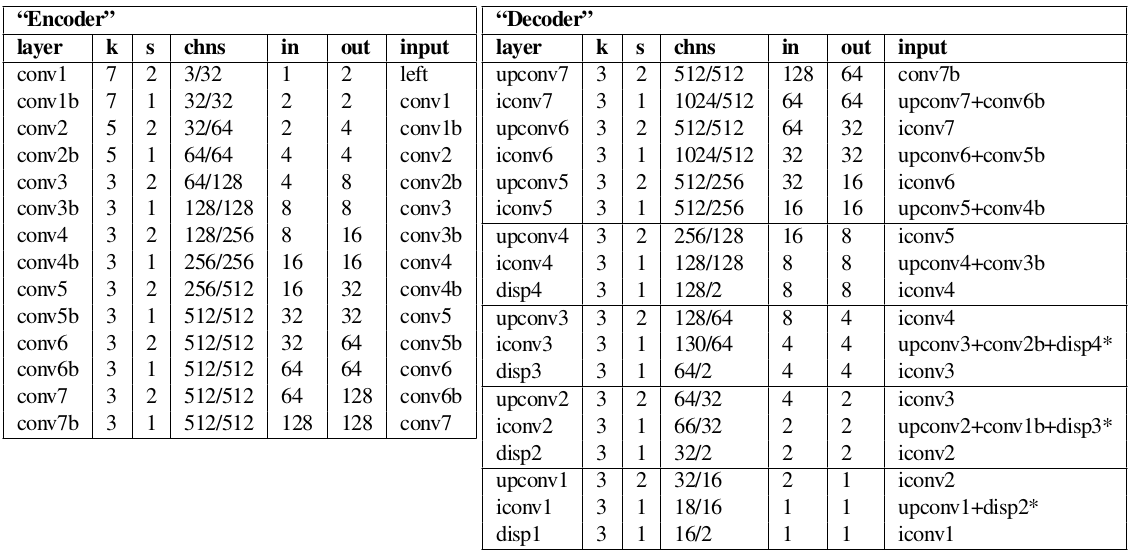
\includegraphics[width=350px]{arch.png}
%	%\fbox{\rule[-.5cm]{0cm}{4cm} \rule[-.5cm]{4cm}{0cm}}
%	\caption{Network architecture.}
%\end{figure}

\bibliography{ref}

\end{document}